\documentclass[uplatex,12pt,dvipdfmx]{jsarticle}

\usepackage{fullpage}
\usepackage{amsmath, amssymb, amsthm}
\usepackage{mathtools}
\usepackage{stmaryrd}

\usepackage[unicode,pagebackref]{hyperref} 
\usepackage{url}
\hypersetup{breaklinks=true}

\usepackage[all]{xy}

\usepackage{tikz}
\usetikzlibrary{matrix}
\usepackage{dynkin-diagrams}

\usepackage{empheq}


\makeatletter
\def\lst@lettertrue{\let\lst@ifletter\iffalse}
\makeatother


\setcounter{MaxMatrixCols}{20}

\theoremstyle{definition}
\newtheorem{definition}{Definition}[section]
\newtheorem{theorem}[definition]{Theorem}
\newtheorem{proposition}[definition]{Proposition}
\newtheorem{lemma}[definition]{Lemma}
\newtheorem{remark}[definition]{Remark}
\newtheorem{example}[definition]{Example}
\newtheorem{main}[definition]{Main Theorem}
\newtheorem{question}[definition]{Question}

\numberwithin{equation}{section}

\newcounter{proofcounter}[definition]

\makeatletter
\renewenvironment{proof}[1][Proof.]{\par
	\pushQED{\qed}%
	\normalfont \topsep6\p@\@plus6\p@\relax
	\trivlist
	\refstepcounter{proofcounter} %proof環境用カウンタをインクリメント
	\item[\hskip\labelsep
	\bfseries
	#1\@addpunct{.}]\ignorespaces
}{%
	\popQED\endtrivlist\@endpefalse
}


\newcommand{\Z}{\mathbb{Z}}
\newcommand{\Real}{\mathbb{R}}
\newcommand{\Complex}{\mathbb{C}}
\newcommand{\Projective}{\mathbb{P}}
\DeclareMathOperator{\linearspan}{span}
\newcommand{\Vect}{\mathrm{Vect}}
\newcommand{\Rep}{\mathrm{Rep}}
\DeclareMathOperator{\Image}{Im}
\DeclareMathOperator{\Kernel}{Ker}
\DeclareMathOperator{\length}{\ell}
\DeclareMathOperator{\Sym}{Sym}
\DeclareMathOperator{\rank}{rank}
\DeclarePairedDelimiter{\abra}{\langle}{\rangle} % < > angle brackets
\DeclarePairedDelimiter{\abs}{\lvert}{\rvert} % | | absolute value
\DeclarePairedDelimiter{\rbra}{\lparen}{\rparen} % () round brackets
\DeclarePairedDelimiter{\cbra}{\lbrace}{\rbrace} % {} curly brackets
\DeclarePairedDelimiter{\ssbra}{\llbracket}{\rrbracket} % [[]] double square brackets
\newcommand{\Eulercharacteristic}{\chi}
\newcommand{\Chernclass}{c}
\DeclareMathOperator{\Picard}{Pic}

\newcommand{\numGrothendieckgrp}[1]{K({#1})_{\mathrm{num}}}%numerical Grothendieck group
\newcommand{\transpose}[1]{{\vphantom{#1}}^t \hspace{-1pt}#1}


\allowdisplaybreaks

\newcommand{\Hline}[1]{\noalign{\hrule height #1}}

\newcommand{\relmiddle}[1]{\mathrel{}\middle#1\mathrel{}}

\title{}
\date{\empty}
\author{}


\begin{document}

\maketitle

\section{Markov 方程式}

\cite{devolcsey2016analoguemarkovequationexceptional}で次の Serre lattice が定義されている。

\begin{definition}
	Serre lattice $(K, \abra{\text{--}, \text{--}}, s)$とは、
	\begin{itemize}
		\item $K$: free abelian group of finite rank, 
		\item $\abra{\text{--}, \text{--}}$: $K$上のnondegenerate bilinear form, 
		\item $s$: $K$上のautomorphism
	\end{itemize}
	の組であり、
	\begin{align}
		\forall u, v\in K, \abra{u, v}=\abra{v, su}
	\end{align}
	が成り立つもののことをいう。
\end{definition}

$X$ を smooth projective threefold, $\numGrothendieckgrp{X}$ をその numerical Grothendieck group, $s$ を Serre functor が誘導する $\numGrothendieckgrp{X}$ 上の automorphism とする。
このとき $\numGrothendieckgrp{X}$ は Euler form から誘導される nondegenerate bilinear form $\abra{\text{--}, \text{--}}$ と Serre functor から誘導される $\numGrothendieckgrp{X}$ 上の automorphism $s$ を備えた Serre lattice となる。

また、{\cite[Proposition 2.1]{devolcsey2016analoguemarkovequationexceptional}}から
\begin{align}
	(s + 1)^4 = ((-1)^3 s - 1)^{3 + 1}=0
\end{align}
が成立する。

$K$ は rank $n$ の Serre lattice であるとする。
$K$ の $\Z$-basis $(e_i)_{i=1}^n$ に対して Gram matrix
\begin{align}
	M=\begin{pmatrix}
		\abra{e_1, e_1}&\cdots&\abra{e_1, e_n}\\
		\cdots&\cdots&\cdots\\
		\abra{e_n, e_1}&\cdots&\abra{e_n, e_n}
	\end{pmatrix}\in M_n(\Z)
\end{align}
を考える。
$s$ の行列表示 $S$ を
\begin{align}
	\begin{pmatrix}
		se_1&\cdots&se_n
	\end{pmatrix}=\begin{pmatrix}
		e_1&\cdots&e_n
	\end{pmatrix}S
\end{align}
で定めると
\begin{align}
	S=M^{-1}\transpose{M}
\end{align}
が成立する。

$n=4$ で $(e_i)_{i=1}^4$ が exceptional basis, つまり $M$ が対角成分1の上三角行列である場合を考える。
\begin{align*}
	M = \begin{pmatrix}
		1&a&b&c\\
		0&1&d&e\\
		0&0&1&f\\
		0&0&0&1
	\end{pmatrix}\in M_4(\Z)
\end{align*}
とおく。
このとき{\cite[Lem 3.1.3]{devolcsey2016analoguemarkovequationexceptional}}の類似で次が成立する。
\begin{proposition}
	\begin{gather}
		q_1(M) = acdf - abd - ace - bcf - def + a^2 + b^2 + c^2 + d^2 + e^2 + f^2, \\
		q_2(M) = af - be + cd
	\end{gather}
	とおくとき、
	\begin{align}
		(s + 1)^4 = 0
	\end{align}
	が成り立つための必要十分条件は $M$ が次のディオファントス方程式の解であることである。
	\begin{subequations}\label{markov_eq}
		\begin{empheq}[left = {\empheqlbrace \, }, right = {}]{align}
			& q_1(M) = 8\\
			& q_2(M)^2 = 16
		\end{empheq}.
	\end{subequations}
\end{proposition}

\begin{proof}
	$S$ の固有多項式 $\chi(t) = \det(tI - S)$ を考える。
	\begin{align}
		\chi(t) = \det(tI - S) = \det(tI - M^{-1}\transpose{M}) = (\det M^{-1})\det(tM - \transpose{M}) = \det(tM - \transpose{M}).
	\end{align}
	
	手計算等で
	\begin{align}
		\det(tM - \transpose{M}) = t^4 + (q_1(M) - 4)t^3 + (q_2(M)^2 - 2q_1(M) + 6)t^2 + (q_1(M) - 4)t + 1
	\end{align}
	が分かるので
	\begin{align}
		(s + 1)^4 = 0\iff&\chi(t) = (t + 1)^4\\
		\iff&q_1(M) - 4 = 4, q_2(M)^2 - 2q_1(M) + 6 = 6\\
		\iff&q_1(M) = 8, q_2(M)^2 = 16.
	\end{align}
\end{proof}

このことから$X$上に長さ4の例外生成列があれば、そのEuler formに関するGram matrixがディオファントス方程式\eqref{markov_eq}の解となることが分かる。

\section{Exceptional basis全体への作用}

$B_n$ を $n$ 本の紐に関する組み紐群、 $\sigma_1,\ldots,\sigma_{n-1}$ を $B_n$ の基本生成系とする。

$X$ 上に長さ $n$ の例外生成列があるとき、 $i=1,\ldots,n-1$ に対して $\sigma_i$ は $i$, $i+1$ 番目の成分に対するleft mutationとして例外生成列全体に作用する。
$\numGrothendieckgrp{X}$ 上では、 $X$ 上の例外生成列 $(\mathcal{E}_1,\ldots,\mathcal{E}_n)$, $i=1,\ldots,n-1$ に対して
\begin{align}
	\sigma_i\cdot(e_1,\ldots,e_n) = (e_1,\ldots,e_{i-1}, \abra{e_i, e_{i+1}}e_i - e_{i+1}, e_i, e_{i+2},\ldots,e_n)
\end{align}
という作用になる。
ただし $e_i$ は $\mathcal{E}_i$ の $\numGrothendieckgrp{X}$ での像を表す。
これを一般化し、 $B_n$ の Serre lattice の exceptional basis 全体への作用の定義として採用する。
\footnote{\cite{devolcsey2016analoguemarkovequationexceptional}や\cite{MR2084561}では符号が異なり
\begin{align}
	\sigma_i\cdot(e_1,\ldots,e_n) = (e_1,\ldots,e_{i-1}, e_{i+1} - \abra{e_i, e_{i+1}}e_i, e_i, e_{i+2},\ldots,e_n)
\end{align}
で定義している。
このあと見る $q_2$ の符号に関する命題との兼ね合いから、この定義は採用しない。
}
この作用により、exceptional basis から作られる Gram matrix にも $B_n$ の作用が反映される。
$K$ のexceptional basis $(e_1,\ldots,e_n)$ に関する Gram matrix を $M$ とするとき、 $\sigma\in B_n$ に対して $\sigma\cdots(e_1,\ldots,e_n)$ に関する Gram matrix を$\sigma\cdot M$とかくことにする。

$i=1,\ldots,n-1$, $m\in\Z$ に対して
\begin{equation}
	A_j(m)=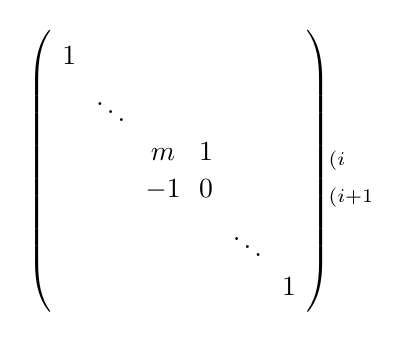
\begin{tikzpicture}[%
		baseline=(m.west),
		every left delimiter/.style={xshift=1ex},
		every right delimiter/.style={xshift=-1ex}]
		\matrix(m)[matrix of math nodes,nodes in empty cells,
		left delimiter={(},right delimiter={)}]
		{
			1 &  &  &  &  &  \\
			& \ddots &  &  &  &  \\
			&  & m & 1 &  &  \\
			&  & -1 & 0 &  &  \\
			&  &  &  & \ddots &  \\
			&  &  &  &  & 1\\
		};
		\node[right=2.5ex]at(m-3-6){${\scriptstyle(i}$};
		\node[right=2.5ex]at(m-4-6){${\scriptstyle(i+1}$};
	\end{tikzpicture}
\end{equation}
と定めるとき、$\forall i=1,\ldots,n-1$ に対して $(e^\prime_1,\ldots,e^\prime_n)=\sigma_i\cdot(e_1,\ldots,e_n)$ とおくと、
\begin{align}
	\begin{pmatrix}
		e^\prime_1&\cdots&e^\prime_n
	\end{pmatrix}=\begin{pmatrix}
		e_1&\cdots&e_n
	\end{pmatrix}A_i(\abra{e_i, e_{i+1}})
\end{align}
が成り立つので
\begin{align}
	\sigma_i\cdot M = \transpose{A_i(\abra{e_i, e_{i+1}})} M A_i(\abra{e_i, e_{i+1}})
\end{align}
という関係が成立する。

$n=4$ の場合を具体的に計算すると次の通り:
\begin{gather}
	\sigma_1 \cdot M = \begin{pmatrix}
		1 & a & ab-d & ac-e \\
		0 & 1 & b & c \\
		0 & 0 & 1 & f \\
		0 & 0 & 0 & 1
	\end{pmatrix},\\
	\sigma_2 \cdot M = \begin{pmatrix}
		1 & ad-b & a & c \\
		0 & 1 & d & de-f \\
		0 & 0 & 1 & e \\
		0 & 0 & 0 & 1
	\end{pmatrix},\\
	\sigma_3 \cdot M = \begin{pmatrix}
		1 & a & fb-c & b \\
		0 & 1 & fd-e & d \\
		0 & 0 & 1 & f \\
		0 & 0 & 0 & 1
	\end{pmatrix}.
\end{gather}

$X$ 上の例外生成列には $\Z^n$ の作用も定義できる。
$\epsilon_1,\ldots,\epsilon_n$ を $\Z^n$ の標準基底とするとき、$X$ 上の例外生成列 $(\mathcal{E}_1,\ldots,\mathcal{E}_n)$, $i=1,\ldots,n-1$ に対して
\[ \epsilon_i\cdot(\mathcal{E}_1,\ldots,\mathcal{E}_n)=(\mathcal{E}_1,\ldots,\mathcal{E}_{i-1},\mathcal{E}_i[1],\mathcal{E}_{i+1},\ldots,\mathcal{E}_n) \]
という作用になる。

$\numGrothendieckgrp{X}$ 上では shift functor は $(-1)$ 倍することに対応し、
\begin{align}
	\epsilon_i\cdot(e_1,\ldots,e_n) = (e_1,\ldots,e_{i-1}, -e_i, e_{i+1},\ldots,e_n)
\end{align}
という作用になる。
ただし $e_i$ は $\mathcal{E}_i$ の $\numGrothendieckgrp{X}$ での像を表す。
これを一般化し、$\Z^n$ の Serre lattice の exceptional basis 全体への作用の定義として採用する。
\footnote{本質的には $(\Z/2\Z)^n$ の作用となる。}
この作用により、exceptional basis から作られる Gram matrix にも $\Z^n$ の作用が反映される。
$K$ の exceptional basis $(e_1,\ldots,e_n)$ に関する Gram matrix を $M$ とするとき、$v\in B_n$ に対して $v\cdots(e_1,\ldots,e_n)$ に関する Gram matrix を $v\cdot M$ とかくことにする。

$n=4$ の場合を具体的に計算すると次の通り:
\begin{gather}
	\epsilon_1 \cdot M = \begin{pmatrix}
		1 & -a & -b & -c \\
		0 & 1 & d & e \\
		0 & 0 & 1 & f \\
		0 & 0 & 0 & 1
	\end{pmatrix},\\
	\epsilon_2 \cdot M = \begin{pmatrix}
		1 & -a & b & c \\
		0 & 1 & -d & -e \\
		0 & 0 & 1 & f \\
		0 & 0 & 0 & 1
	\end{pmatrix},\\
	\epsilon_3 \cdot M = \begin{pmatrix}
		1 & a & -b & c \\
		0 & 1 & -d & e \\
		0 & 0 & 1 & -f \\
		0 & 0 & 0 & 1
	\end{pmatrix},\\
	\epsilon_4 \cdot M = \begin{pmatrix}
		1 & a & b & -c \\
		0 & 1 & d & -e \\
		0 & 0 & 1 & -f \\
		0 & 0 & 0 & 1
	\end{pmatrix}.
\end{gather}

以上で $B_n\ltimes\Z^n$ の作用が定義された。

$n=4$ で $(s + 1)^4 = 0$ が成立する場合は $\forall\sigma\in B_4\ltimes\Z^4$ に対して $\sigma\cdot M$ もディオファントス方程式\eqref{markov_eq}の解となる。
このうち、$q_2$ については $4,-4$ の 2 通りの値を取り得るが、 $B_n$ の作用では $q_2$ は保存される。
一方、$\epsilon_1,\epsilon_2,\epsilon_3,\epsilon_4$ の作用では符号が反転する。

\begin{proposition}
	$K$ は Serre lattice of rank $4$ であるとする。
	このとき $\forall\sigma\in B_n$ について
	\begin{align*}
		q_2(\sigma\cdot M) = q_2(M)
	\end{align*}
	が成立する。
\end{proposition}

\begin{proof}
	手計算で $\sigma_1\cdot M,\sigma_2\cdot M,\sigma_3\cdot M$ について成立することが分かる。
\end{proof}

\begin{proposition}
	$K$ は Serre lattice of rank $4$ であるとする。
	このとき $\forall i=1,2,3,4$ について
	\begin{align*}
		q_2(\epsilon_i\cdot M) = -q_2(M)
	\end{align*}
	が成立する。
\end{proposition}

\begin{proof}
	手計算で成立することが分かる。
\end{proof}


以上でディオファントス方程式\eqref{markov_eq}の解に対する $B_4\ltimes\Z^4$ の作用が定義された。

\section{4つのthreefold}

{\cite[Lemma 3.5]{nordskova2025exceptionalcollectionsfanothreefolds}}によると 4 つのベクトル束からなる例外生成列を持つ smooth projective threefold は $X = \Projective^3,Q_3,V_5,V_{22}$ に限られる。
これらの例外生成列からディオファントス方程式\eqref{markov_eq}の解の系列が得られる。
例外生成列をひとつ列挙し、その系列の代表系となるGram matrixを計算する。

\subsection{$\Projective^3$}

\cite{MR509388}で $(\mathcal{O}_{\Projective^n}, \mathcal{O}_{\Projective^n}(1), \ldots, \mathcal{O}_{\Projective^n}(n))$ は $\Projective^n$ の例外生成列であることが示されている。
特に $(\mathcal{O}_{\Projective^3}, \mathcal{O}_{\Projective^3}(1), \mathcal{O}_{\Projective^3}(2), \mathcal{O}_{\Projective^3}(3))$ は $\Projective^3$ の例外生成列となる。
Gram matrixは
\begin{gather}
	M_{\mathbb{P}^3} = \begin{pmatrix}
		1 & 4 & 10 & 20 \\
		0 & 1 & 4 & 10 \\
		0 & 0 & 1 & 4 \\
		0 & 0 & 0 & 1
	\end{pmatrix},\\
	q_2(M_{\mathbb{P}^3}) = -4
\end{gather}
となる。

\subsection{$Q_3$}

$\Projective^{n+1}$ 内の $2$ 次超曲面を$Q_n$とかく。
$n$が奇数のとき、$n = 2k + 1$ とおくと、$Q_n$は$B_{k+1}$型の単連結複素単純 Lie 群 $G = Spin(2k + 3)$ の旗多様体とみなせる。
対応する crossed out Dynkin diagram は $\dynkin[labels={\alpha_1,,,\alpha_{k+1}}] B{x*...**}$となる。

最高ウェイトが$(0,\ldots,0,1)$\footnote{メモ:小林さんのパッケージでの最高ウェイト}である$Q_n$上の同変ベクトル束を$\Sigma$とかくことにする。
$\Sigma$はスピノル束と呼ばれている。
このとき $(\mathcal{O}_{Q_3}(-2), \mathcal{O}_{Q_3}(-1), \mathcal{O}_{Q_3}, \Sigma)$ は $Q_3$ の例外生成列であることが\cite{MR939472}で示されている。
\footnote{メモ:\cite{ABondal1995SemiorthogonalDF}でもそのように引用されている。}
Gram matrixは
\begin{gather}
	M_{Q_3} = \begin{pmatrix}
		1 & \Eulercharacteristic(\mathcal{O}_{Q_3}(1)) & \Eulercharacteristic(\mathcal{O}_{Q_3}(2)) & \Eulercharacteristic(\Sigma(2)) \\
		0 & 1 & \Eulercharacteristic(\mathcal{O}_{Q_3}(1)) & \Eulercharacteristic(\Sigma(1)) \\
		0 & 0 & 1 & \Eulercharacteristic(\Sigma) \\
		0 & 0 & 0 & 1
	\end{pmatrix} = \begin{pmatrix}
		1 & 5 & 14 & 40 \\
		0 & 1 & 5 & 16 \\
		0 & 0 & 1 & 4 \\
		0 & 0 & 0 & 1
	\end{pmatrix},\\
	q_2(M_{Q_3}) = -4
\end{gather}
となる。
\footnote{$\mathcal{O}_{Q_3}(1)$ が最高ウェイト $(1, 0)$ に対応し、$\mathcal{O}_{Q_3}(2)$, $\Sigma$, $\Sigma(1)$, $\Sigma(2)$ もそれぞれ $(2, 0)$, $(0, 1)$, $(1, 1)$, $(2, 1)$ に対応する。
小林さんパッケージ(を少し修正したもの)で計算してみた結果となる。
Geminiの主張とも一致する。}


\subsection{$V_5$}

$V_5$ とは、Grassmann 多様体 $Gr(2,5)$ の一般的な 3 つの超平面断面として実現される Fano threefold である。

$Gr(2,5)$ は $A_4$型の $SL(5,\Complex)$ の旗多様体であり、対応する crossed out Dynkin diagram は $\dynkin[labels={\alpha_1,\alpha_2,\alpha_3,\alpha_4}] A{*x**}$となる。
$\mathcal{U}$ を $Gr(2,5)$ 上の tautological bundle を $V_5$ に制限したものとする。
このとき $(\mathcal{O}_{V_5}, \mathcal{U}^*, \mathcal{O}_{V_5}(1), \mathcal{U}^*(1))$ は $V_5$ の例外生成列であることが\cite{MR1294662}で示されている。
Gram matrixは
\begin{gather}
	M_{V_5} = \begin{pmatrix}
		1 & \Eulercharacteristic(\mathcal{U}^*) & \Eulercharacteristic(\mathcal{O}_{V_5}(1)) & \Eulercharacteristic(\mathcal{U}^*(1)) \\
		0 & 1 & \Eulercharacteristic(\mathcal{U}(1)) & \Eulercharacteristic(\mathcal{U}\otimes\mathcal{U}^*(1)) \\
		0 & 0 & 1 & \Eulercharacteristic(\mathcal{U}^*) \\
		0 & 0 & 0 & 1
	\end{pmatrix} = \begin{pmatrix}
		1 & 5 & 7 & 25 \\
		0 & 1 & 5 & 22 \\
		0 & 0 & 1 & 5 \\
		0 & 0 & 0 & 1
	\end{pmatrix},\\
	q_2(M_{V_5}) = -4
\end{gather}
となる。
\footnote{$\mathcal{O}_{V_5}(1)$ が最高ウェイト $(0, 1, 0, 0)$, $\mathcal{U}^*$ が$(1, 0, 0, 0)$に対応する。
小林さんのパッケージによる計算結果であり、Geminiの主張とも一致する。}

\subsection{$V_{22}$}

$V_{22}$ とは、$Gr(3, 7)$ 上の tautological bundle を $\mathcal{U}$ とするとき、$(\bigwedge^2 \mathcal{U}^\vee)^{\oplus3}$の一般切断として実現される Fano threefold である。

$Gr(3,7)$ は $A_6$型の $SL(7,\Complex)$ の旗多様体であり、対応する crossed out Dynkin diagram は $\dynkin[labels={\alpha_1,\alpha_2,\alpha_3,\alpha_4,\alpha_5,\alpha_6}] A{**x***}$となる。
このとき rank $2$のベクトル束$\mathcal{E}$
\footnote{Mukai bundleとよばれている。
	$V_{22}$ の超平面切断 $Y$ 上の直線束 $\mathcal{O}_Y(L)$ に付随して定義される束で、以下の完全列を満たす核として定義される。
	\begin{align}
		\xymatrix{
			0 \ar[r] &\mathcal{E} \ar[r]& H^0(\mathcal{O}_Y(L)) \otimes \mathcal{O}_X \ar[r]& \mathcal{O}_Y(L) \ar[r]& 0
		}.
	\end{align}
	ここで $L$ は $V_{22}$ 上の直線を表す。
	また、双対束 $\mathcal{E}^\vee$ は $\mathcal{E} \otimes \mathcal{O}_X(-K_X)$ と同型になる。
}
が存在して $\mathcal{U}$ は $V_{22}$ に制限したものを意味するとして $(\mathcal{O}_{V_{22}}, \mathcal{U}^*, \mathcal{E}^*, \bigwedge^2 \mathcal{U}^*)$ は $V_{22}$ の例外生成列であることが\cite{MR1445274}で示されている。

ただし、GeminiとSageMathによる計算結果によれば$\mathcal{E}$は$K$群において
\begin{align}
	[\mathcal{E}^\vee] = -\frac{1}{20}[\mathcal{O}_{V_{22}}] + \frac{7}{20}[\mathcal{U}^*] + \frac{7}{20}[\bigwedge^2 \mathcal{U}^*] - \frac{1}{20}[\mathcal{O}_{V_{22}}(1)]
\end{align}
を満たすベクトル束らしい。
Gram matrixは
\begin{gather}
	M_{V_{22}} = \begin{pmatrix}
		1 & \Eulercharacteristic(\mathcal{U}^*) & \Eulercharacteristic(\mathcal{E}^*) & \Eulercharacteristic(\bigwedge^2 \mathcal{U}^*) \\
		0 & 1 & \Eulercharacteristic(\mathcal{U}\otimes\mathcal{E}^*) & \Eulercharacteristic(\mathcal{U}\otimes\bigwedge^2 \mathcal{U}^*) \\
		0 & 0 & 1 & \Eulercharacteristic(\mathcal{E}\otimes\bigwedge^2 \mathcal{U}^*) \\
		0 & 0 & 0 & 1
	\end{pmatrix} = \begin{pmatrix}
		1 & 7 & 8 & 18 \\
		0 & 1 & 4 & 13 \\
		0 & 0 & 1 & 4 \\
		0 & 0 & 0 & 1
	\end{pmatrix},\\
	q_2(M_{V_{22}}) = -4
\end{gather}
となる。
\footnote{$\mathcal{U}^*$ は $(1, 0, 0, 0, 0, 0)$ に対応する。}

\begin{question}
	ディオファントス方程式\eqref{markov_eq}の解の $B_n\ltimes\Z^n$ あるいは $B_n$ による orbit は $\Projective^3$, $Q_3$, $V_5$, $V_{22}$ のもので尽きるか?
	また、これらは異なる orbit を成すか?
\end{question}

\section{数値的解の探索と独立性の証明}

計算機探索により、既知の4つの多様体($\Projective^3, Q_3, V_5, V_{22}$)のいずれの軌道にも属さない数値的解(Numerical Solution)の存在が確認された。
以下にその具体例と、独立性の証明を与える。

\subsection{数値的解の発見}
成分の絶対値が小さい範囲での全探索により、多数の新しい解が見出された。
その中でも最小のノルム(非対角成分の二乗和の平方根)を持つ例として、以下の行列 $M_{\mathrm{ghost}}$ を挙げる。

\begin{align}
    M_{\mathrm{ghost}} = \begin{pmatrix}
        1 & 0 & 0 & 0 \\
        0 & 1 & -2 & -2 \\
        0 & 0 & 1 & 0 \\
        0 & 0 & 0 & 1
    \end{pmatrix}
\end{align}

この行列の不変量は $q_1(M_{\mathrm{ghost}}) = 8, q_2(M_{\mathrm{ghost}}) = 4$ であり、Markov型方程式の条件を満たす。

\subsection{別軌道であることの証明}

発見された解 $M_{\mathrm{ghost}}$ が、既知の4つの多様体の軌道 $O_{X}$ ($X \in \{\Projective^3, Q_3, V_5, V_{22}\}$) のいずれにも含まれないことを、有限体 $\mathbb{F}_3$ 上への還元を用いて証明する。

\begin{theorem}
    数値的解 $M_{\mathrm{ghost}}$ は、$\Projective^3, Q_3, V_5, V_{22}$ のいずれの $B_n\ltimes\Z^n$ 軌道にも属さない。
\end{theorem}

\begin{proof}
    もし $M_{\mathrm{ghost}}$ がある多様体 $X$ の軌道 $O_X$ に含まれるならば、任意の素数 $p$ に対して、法 $p$ で還元した行列も対応する軌道 $\overline{O_X}^{(p)}$ に含まれなければならない。
    
    $p=3$ において、各多様体の軌道全体 $\overline{O_X}^{(3)}$ を計算機により生成したところ、その要素数は以下の通りであった。
    \begin{itemize}
        \item $|\overline{O_{\Projective^3}}^{(3)}| = 216$
        \item $|\overline{O_{Q_3}}^{(3)}| = 8$
        \item $|\overline{O_{V_5}}^{(3)}| = 216$
        \item $|\overline{O_{V_{22}}}^{(3)}| = 216$
    \end{itemize}
    
    一方、$M_{\mathrm{ghost}}$ を法 $3$ で還元すると
    \begin{align}
        M_{\mathrm{ghost}} \equiv \begin{pmatrix}
            1 & 0 & 0 & 0 \\
            0 & 1 & 1 & 1 \\
            0 & 0 & 1 & 0 \\
            0 & 0 & 0 & 1
        \end{pmatrix} \pmod 3
    \end{align}
    となる。この行列は、上で生成したどの集合 $\overline{O_X}^{(3)}$ にも含まれないことが確認された。
    したがって、対偶により $M_{\mathrm{ghost}}$ は整数環 $\Z$ 上において、これら4つの多様体のどの軌道にも属さない。
\end{proof}

なお、同様の方法で他の数値的解についても独立性を確認している。

また、modulo 6での軌道の要素数から$\Projective^3, Q_3, V_5, V_{22}$の軌道が互いに異なることも確認できる。

\subsection{結論}
以上の結果より、方程式\eqref{markov_eq}の整数解の軌道は、既知のFano 3-fold由来の4つの系列だけでは尽くされないことが示された。
今回発見された数値的解は、幾何学的な背景を持たない(あるいは未知の幾何学的対象に対応する)「幽霊解(Phantom Solution)」であると考えられる。

そこで、次の問題を考える。

\begin{question}
	ディオファントス方程式\eqref{markov_eq}の解の $B_n\ltimes\Z^n$ あるいは $B_n$ による orbit は無限に存在するか?
\end{question}

\begin{question}
	ディオファントス方程式\eqref{markov_eq}の解の $B_n\ltimes\Z^n$ あるいは $B_n$ による orbit をすべて分類できるか?
\end{question}

\begin{question}
	$B_n\ltimes\Z^n$よりもさらに大きい、由緒正しい群でディオファントス方程式\eqref{markov_eq}の解に作用するものは存在するか?
\end{question}

\begin{question}
	発見された幽霊解に対応する非可換代数幾何学的対象(圏)は構成できるか?
\end{question}

\begin{question}
	数値的解に対応する非可換代数幾何学的対象(圏)の性質はどのようなものか? 例えば、これらの圏の Hochschild ホモロジーや K 群はどのような構造を持つか?
\end{question}

\begin{question}
	幾何的解(ノルム $\geq 136$)と数値的解(ノルム $\leq 44$)の間には、なぜこれほど大きな断絶(ギャップ)があるのか? 中間のノルムを持つ解は存在しないのか?
	※数値解の探索範囲がただ小さいだけと予想されるが、念のため。
\end{question}

\begin{question}
	発見された幽霊解において、Serre functor $S = M^{-1} {}^t M$ のJordan blockのサイズの分布に何か法則はあるか?
\end{question}

\begin{remark}
    いくつかの発見された数値的解 $M_{\mathrm{ghost}}$ について、Serre functor $S = M_{\mathrm{ghost}}^{-1} \transpose{M_{\mathrm{ghost}}}$ のJordan標準形を計算したところ、以下の2種類の異なる構造が見出された。

    \begin{enumerate}
        \item \textbf{Type [4] (Maximally Unipotent):}
        ノルムが $10, 26, 44$ などの解に見られる構造。固有値 $-1$ に対応する $4 \times 4$ のJordanブロックを一つだけ持つ。これは既知のFano 3-foldと同様の性質であり、これらは非可換Fano 3-foldの有力な候補であると考えられる。
        
        \item \textbf{Type [2, 2]:}
        ノルムが $8$ の解(最小ノルム解)に見られる構造。$2 \times 2$ のJordanブロック2つからなる。これは、対応する幾何学的対象が可約であるか、あるいは低次元の対象の積(例えば曲面と曲線の積など)のような構造を持っている可能性を示唆している。
    \end{enumerate}
\end{remark}

\begin{question}
	数値的解の空間は、離散的な点集合に見えるが、これらを結ぶような(複素数体上での)連続的な変形、あるいはモジュライ空間のような構造はあるか?
	(Markov方程式 $x^2+y^2+z^2=3xyz$ は $\mathbb{C}^3$ 上の曲面を定義するが、今回の行列方程式も $\mathbb{C}^{6}$ 内の代数多様体を定義する。その幾何学的性質は?)
\end{question}

\begin{question}
	今回は $n=4$(Fano 3-foldに対応)を扱ったが、$n=5$ の場合に同様の「幽霊解」は現れるか?
\end{question}


\bibliography{reference.bib}
\bibliographystyle{amsalpha}

\end{document}

